\documentclass{article}

% Packages
\usepackage{amsmath}
\usepackage{graphicx}

\begin{document}

\begin{titlepage}
    \centering

    % ---- Title ----
    {\Huge\bfseries NurEngine's Linear Algebra Equator\par}
    \vspace{1.5cm}

    % ---- Authors ----
    {\large
        Rionaldo Casey Pandhitha \\ NIM: 13525030 \\[0.5cm]
        Raffi Fauzi Hermawan \\ NIM: 13525054 \\[0.5cm]
        Fachry Azriel Fajdwani \\ NIM: 13525110 \par
    }
    \vspace{1.5cm}

    % ---- Image ----
    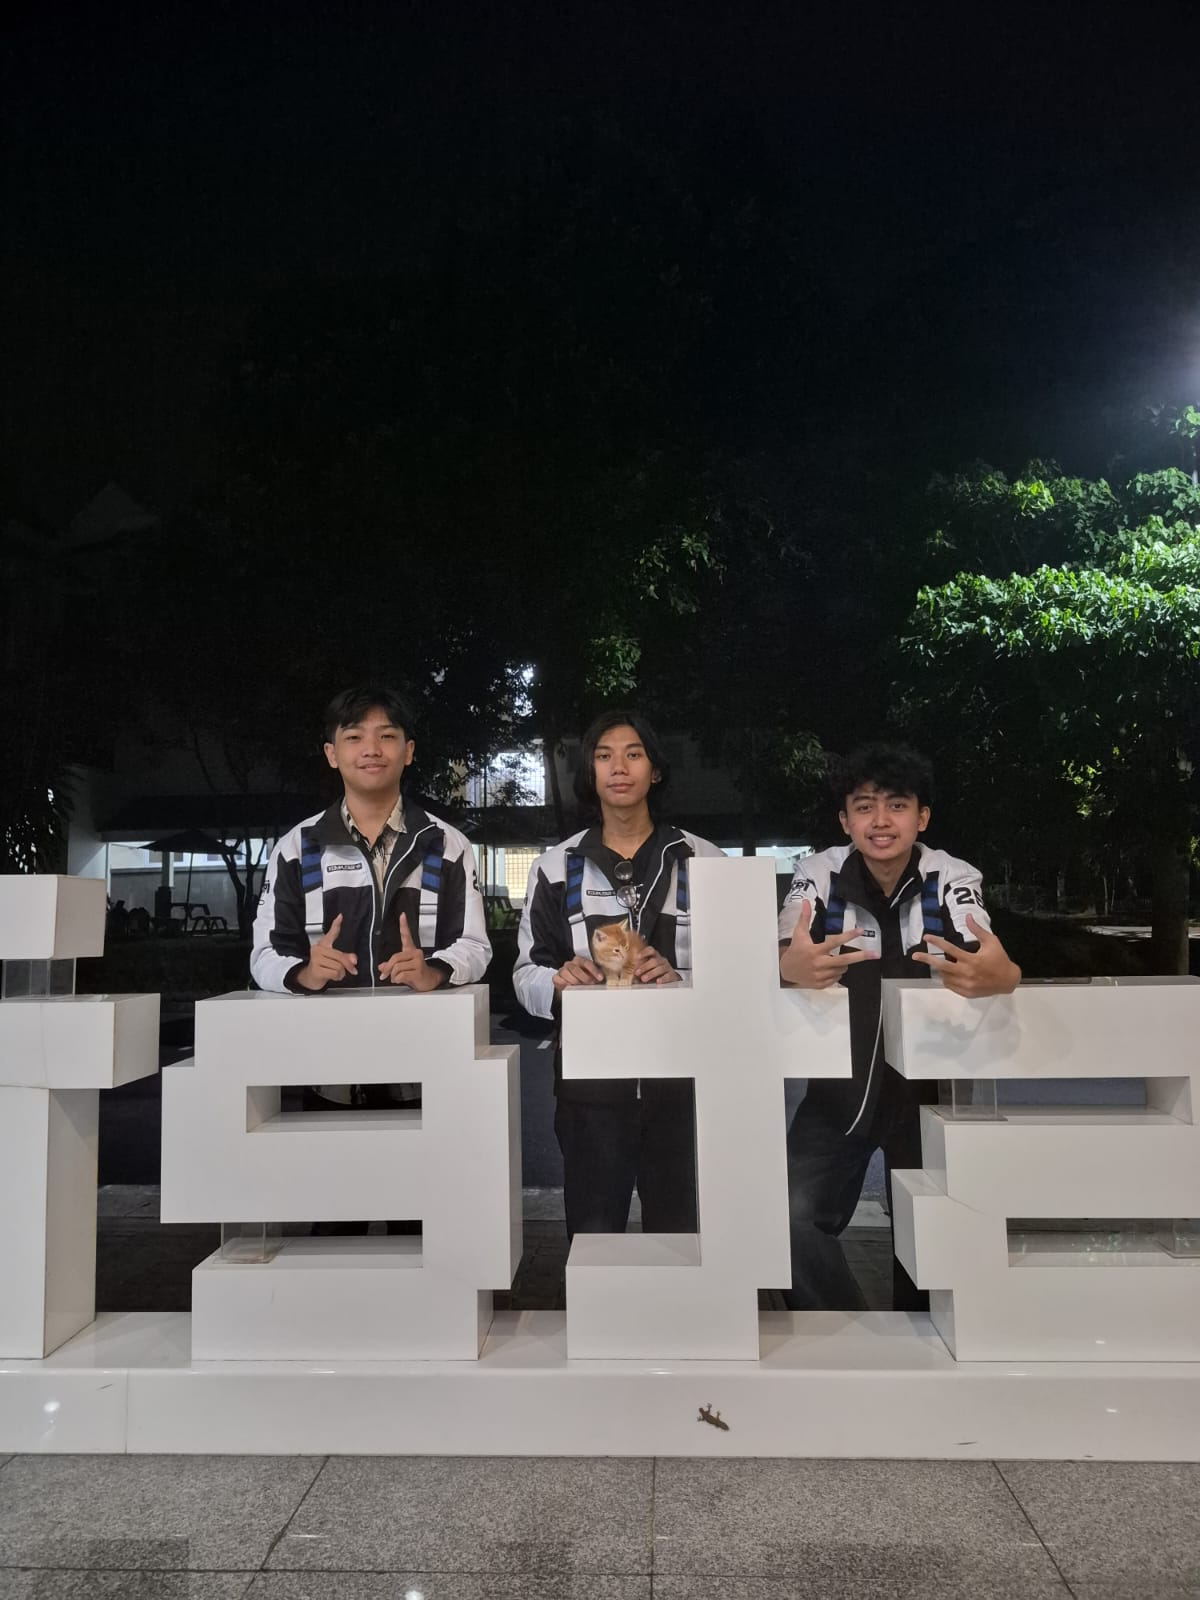
\includegraphics[width=0.55\textwidth]{3_Pria_Hebat.jpg}\\[1cm]

    % ---- Date ----
    {\large \today\par}

\end{titlepage}


\section{Introduction}
This is a simple paragraph of text. LaTeX automatically handles spacing, indentation, and line breaks. You can write normal sentences here, and they will be formatted neatly in the final PDF.

\subsection{Formatting}
You can make text \textbf{bold}, \textit{italic}, or \underline{underlined}. You can also write inline math like $E = mc^2$.

\section{Lists}
Here is a bullet list:
\begin{itemize}
  \item First item
  \item Second item
  \item Third item
\end{itemize}

And here is a numbered list:
\begin{enumerate}
  \item Step one
  \item Step two
  \item Step three
\end{enumerate}

\section{Math}
Inline math: $a^2 + b^2 = c^2$.

Display math:
\begin{equation}
  \int_0^\infty e^{-x^2} \, dx = \frac{\sqrt{\pi}}{2}
\end{equation}

\section{Conclusion}
That's it! Save the file and compile it to see the PDF.

\end{document}